\documentclass[titlepage,twoside,openright,12pt]{article}
\usepackage{graphicx}
\title{Data Structures Final Project}
\author{Cameron Lowell Palmer \and Kristina Ratliff \and Tyler Chamberlain \and Brian Stair}
%\date{}

\begin{document}
\maketitle

\begin{raggedright}

\section*{Introduction}
The problem we were presented with in this project is a difficult one. In fact, it
is characterized as a Steiner tree problem and they are NP-Complete. We discovered
in a paper called \textit{A Fast Algorithm for Steiner Trees}\cite{ks:kmb} a solution that
was implementable and uses algorithms that we studied in the Data Structures course. 
The algorithm is called the KMB algorithm after the initials of the authors. KMB
requires an undirected graph but remains highly useful in solving multicasting 
problems in a reasoable period of time.\\*[1Em]

\section*{KMB Algorithm Steps}
The algorithm can be broken down into the following steps:
\begin{enumerate}
\item Perform Dijkstra's shortest path algorithm on each of the nodes to the other nodes.
\item Using the shortest path information between the starting and ending points create a new graph with just these points and the distance between them.
\item Perform a Minimum Spanning Tree (Kruskal's is used in our implementation) on the graph generated in step two.
\item Reduce the original graph to just the links left by step three.
\item Reduce the graph by MST again to arbitrarily eliminate duplicate links.
\item Construct a Steiner tree by deleting any leftover links (not Steiner points).
\end{enumerate}

\section*{Implementation}
We implemented the program using the Boost (http://www.boost.org/) C++ graph 
libraries, which are currently on a path to be included in the C++ STL. The Boost
libraries are of high quality and are highly regarded in the C++ community. The KMB 
algorithm is not implemented in the Boost libraries, but Dijkstra's and many 
other algorithms are implemented in a very general way. So rather than to use our own 
implementations of Kruskal's algorithm and Dijkstra's shortest path algorithm, 
these guarantee a reasoable running time. Our KMB implementation may take a 
little longer than necessary because we could do a better job of determining 
when Dijkstra's algorithm is finished. Currently, if there are $n$ start and destination 
nodes, we run Dijkstra's algorithm $n$ times. In the case of our basic graph, this includes
one extra run, so larger graphs will have unnecessary computations.\\*[1Em]

The Boost C++ libraries input and output Graphviz natively, which is portable 
across platforms and can easily be converted to PDF. Our output is in PDF form.\\*[1Em]

The exciting thing about this algorithm is how it reduces the graph to a managable
size. The hardest part of determining a shortest path to several nodes is avoiding
looking at every node in the graph. In this algorithm the combination of two well-known 
algorithms yields a good result. We had initially considered several 
algorithms of our own devising, but we always ran into the same problem of high
running times because we were brute-forcing the graph. We spent a lot of time
considering how to reduce the graph in an efficient manner.\\*[1Em]

\section*{Steinlib Graphs}
One of our discoveries was that creating graphs is really hard to do well. When 
you sit down and draw a graph you often substitute spacial randomness for really
complex graphs. We discovered that the Steinlib project provides complex graphs
with large numbers of nodes and edges. A wide variety of Steinlib input files 
can be downloaded from http://elib.zib.de/steinlib/testset.php.

The basic graph provided in the project documentation is used as the example in
this document of input and output. The following section Other Example Graphs are
datasets B01-B05 from Steinlib.

\pagebreak
\begin{verbatim}
33D32945 STP File, STP Format Version 1.0

SECTION Comment
Name    "Project Graph"
Creator "Xiaohui Yuan"
Remark  "The basic project graph"
END

SECTION Graph
Nodes 7
Edges 10
E 0 1 6
E 0 2 2 
E 0 3 1 
E 1 2 3
E 1 4 1
E 2 5 1
E 3 5 3
E 3 6 3
E 4 5 3
E 5 6 2
END

SECTION Terminals
Terminals 3
T 0
T 4
T 6
END

EOF
\end{verbatim}
\begin{center}
\includegraphics[height=3.00in]{project.eps}
\end{center}

\section*{Other Example Graphs}
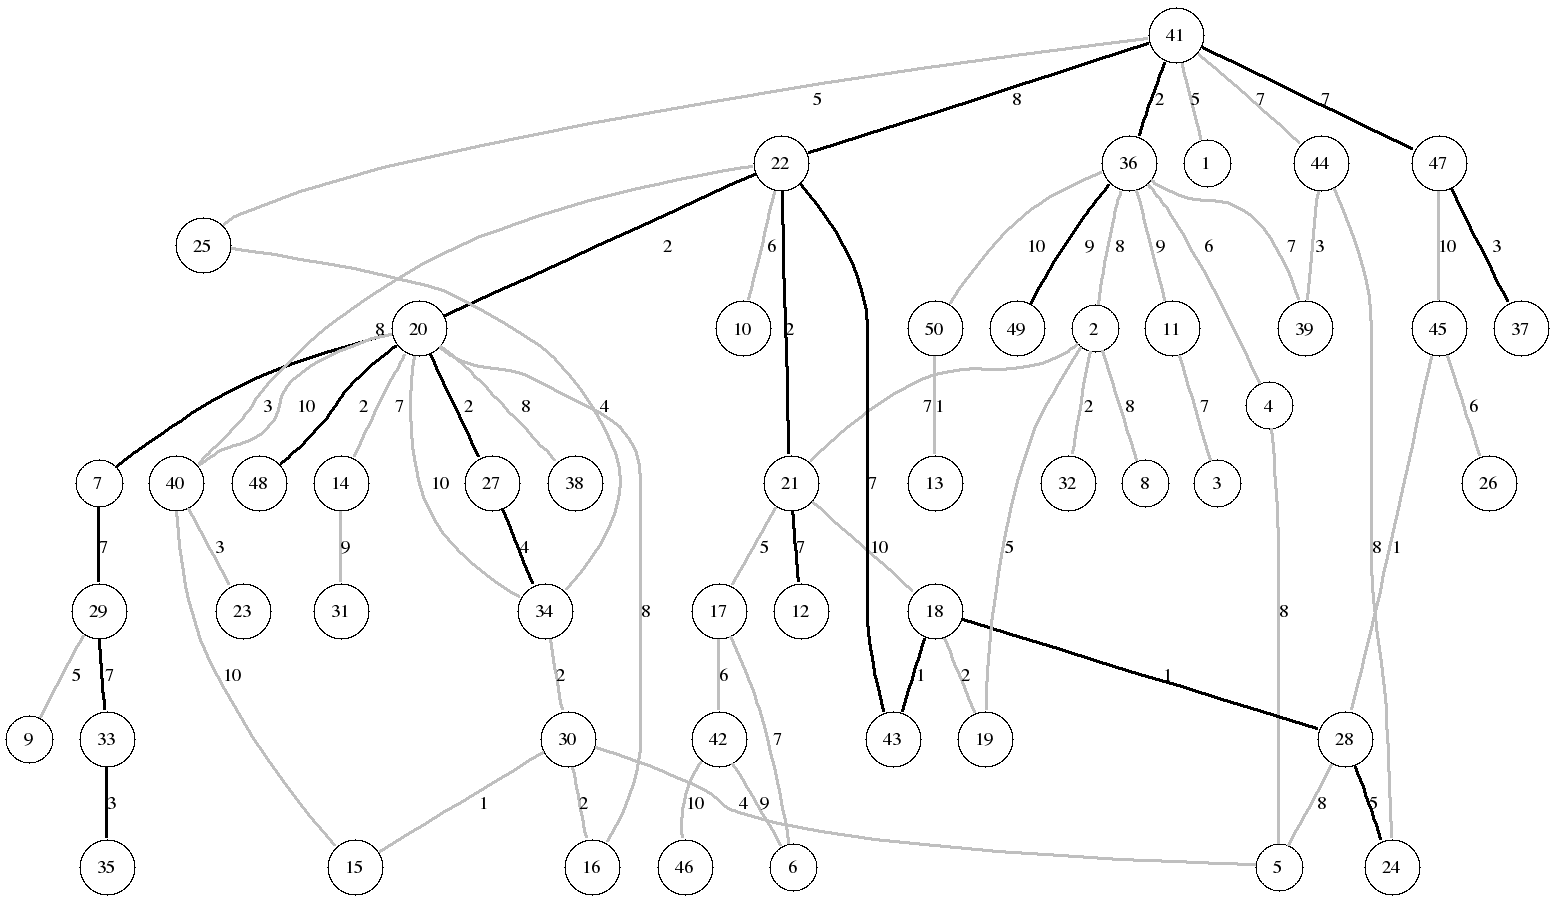
\includegraphics[keepaspectratio=true,width=\linewidth,height=\textheight]{b01.eps}
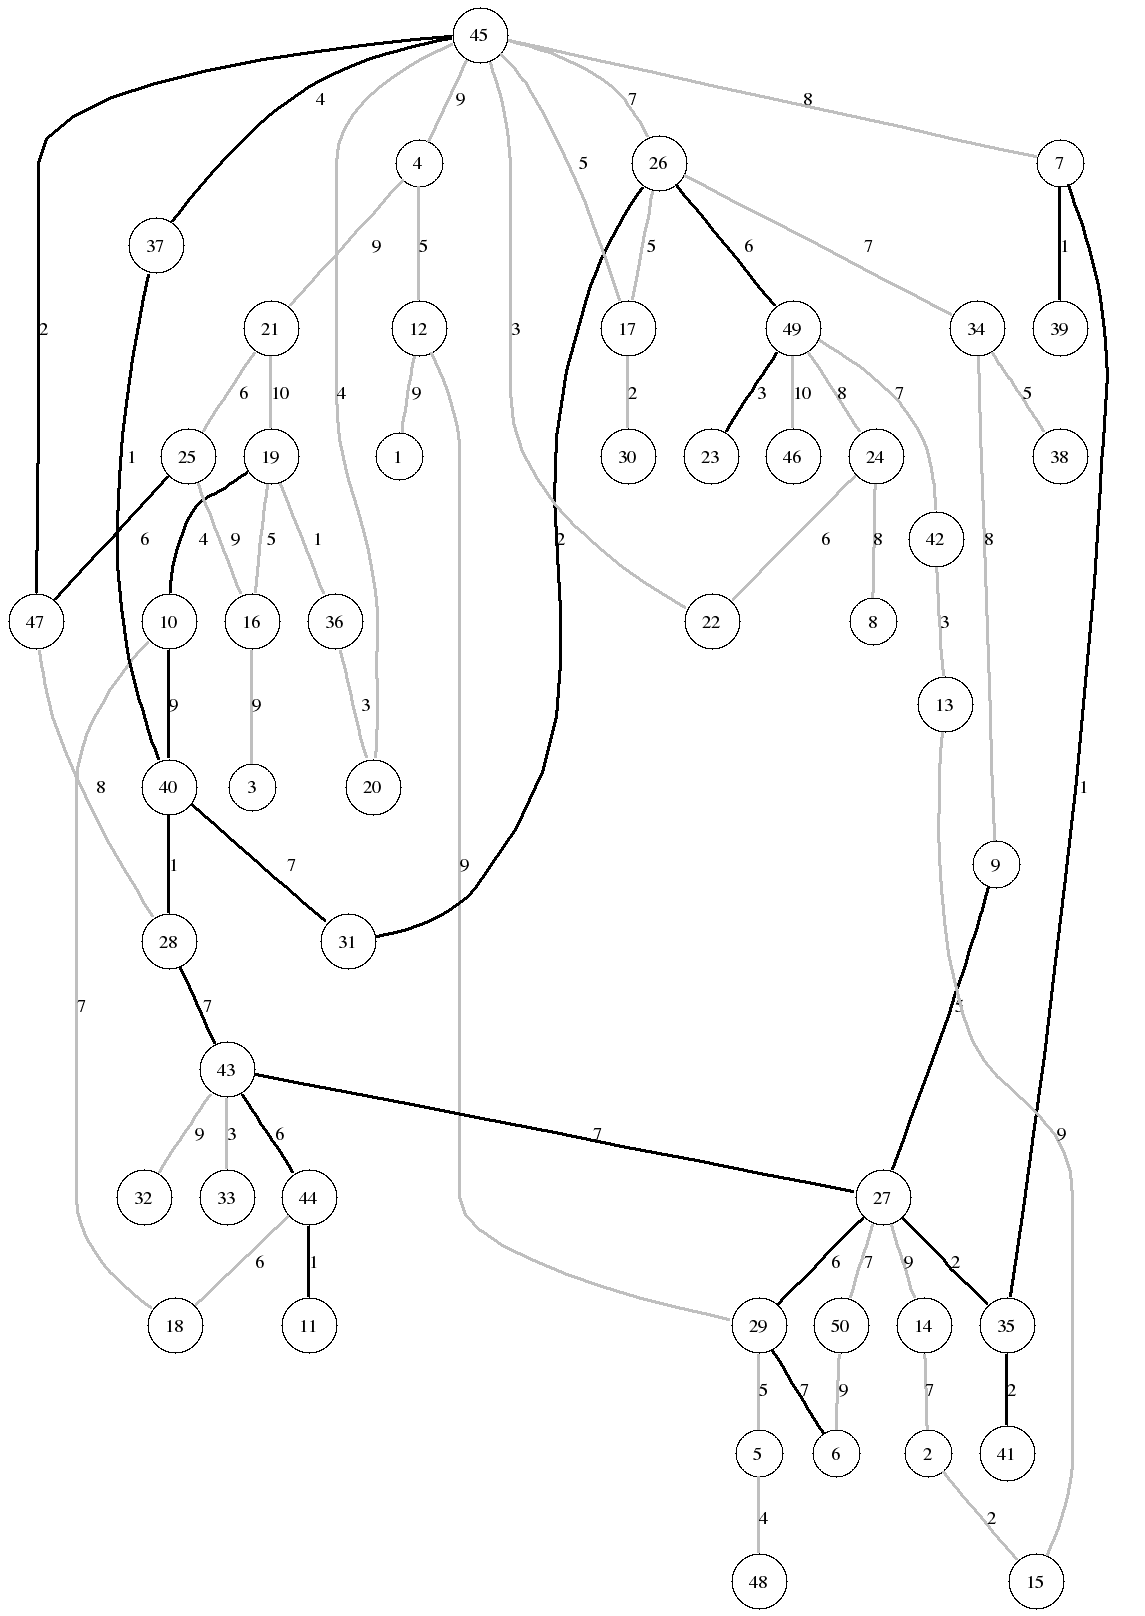
\includegraphics[keepaspectratio=true,width=\linewidth,height=\textheight]{b02.eps}
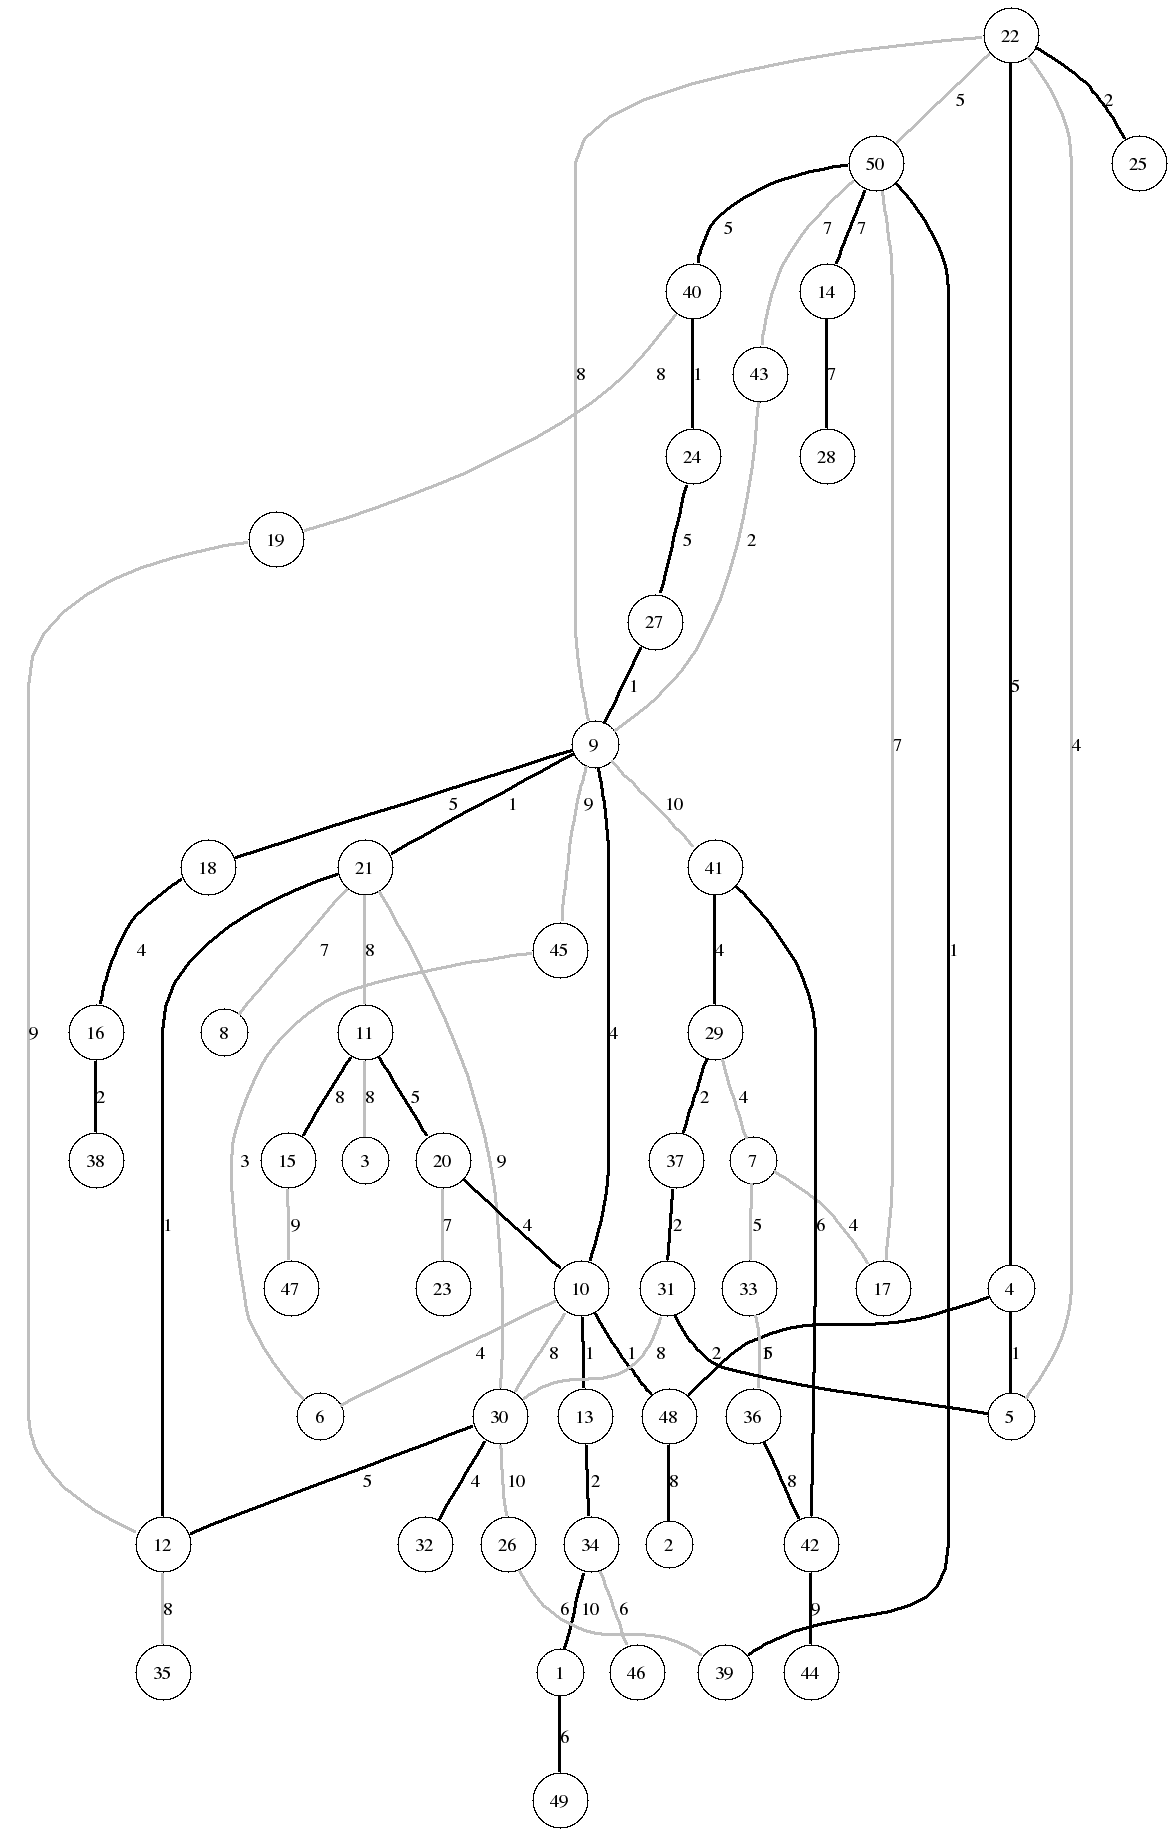
\includegraphics[keepaspectratio=true,width=\linewidth,height=\textheight]{b03.eps}
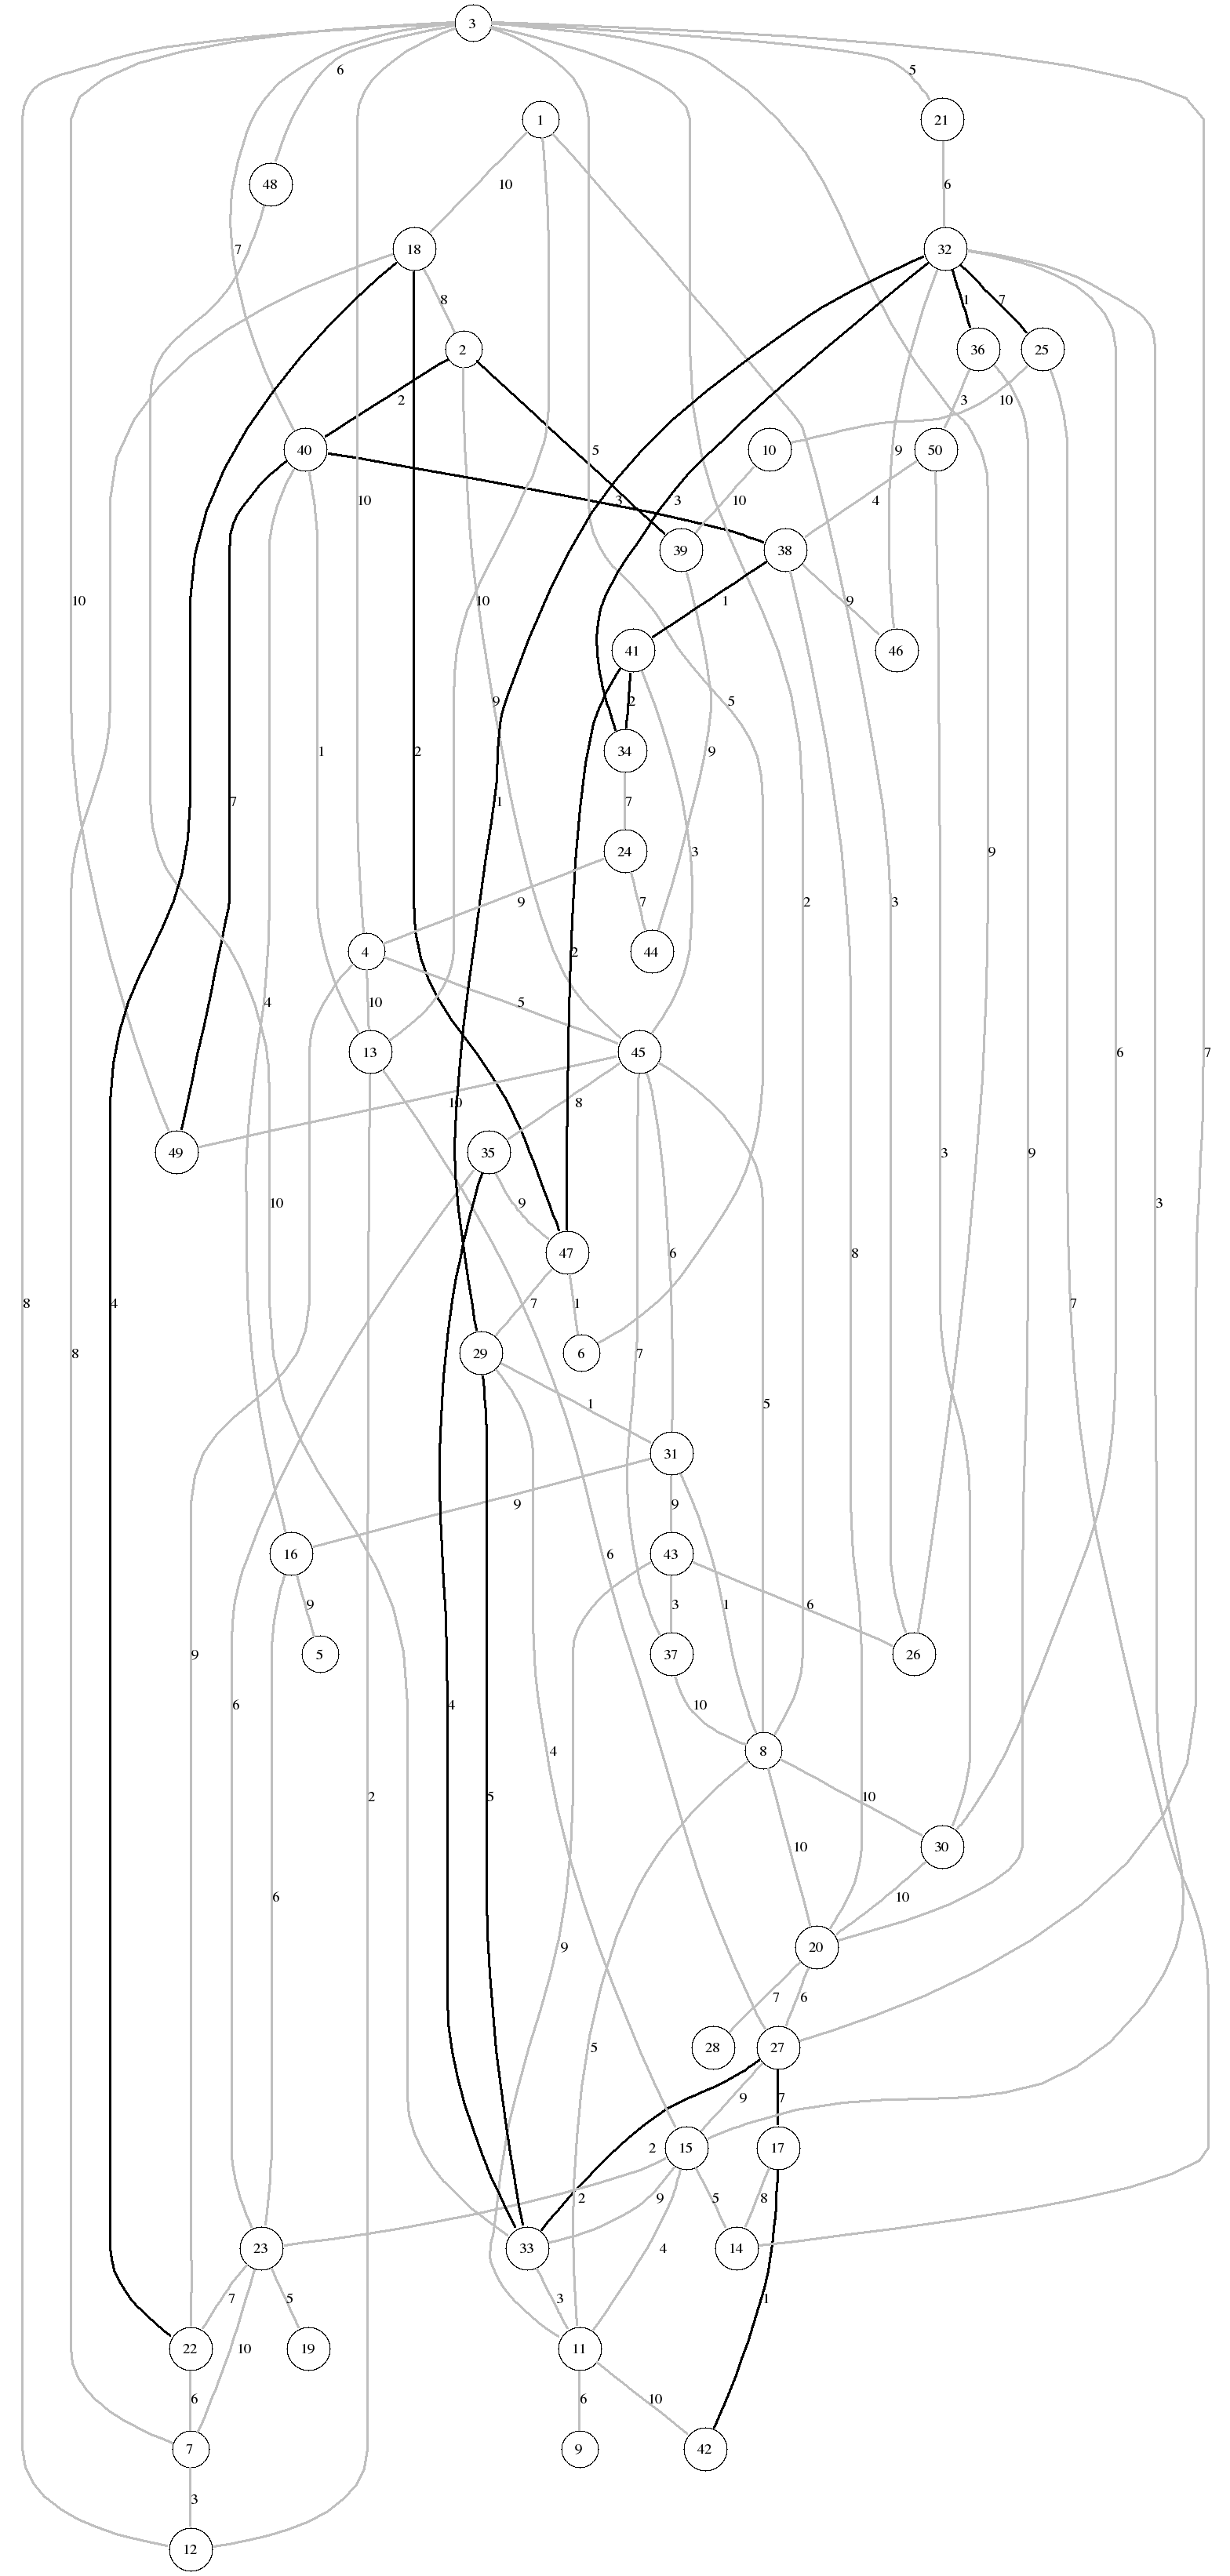
\includegraphics[keepaspectratio=true,width=\linewidth,height=\textheight]{b04.eps}
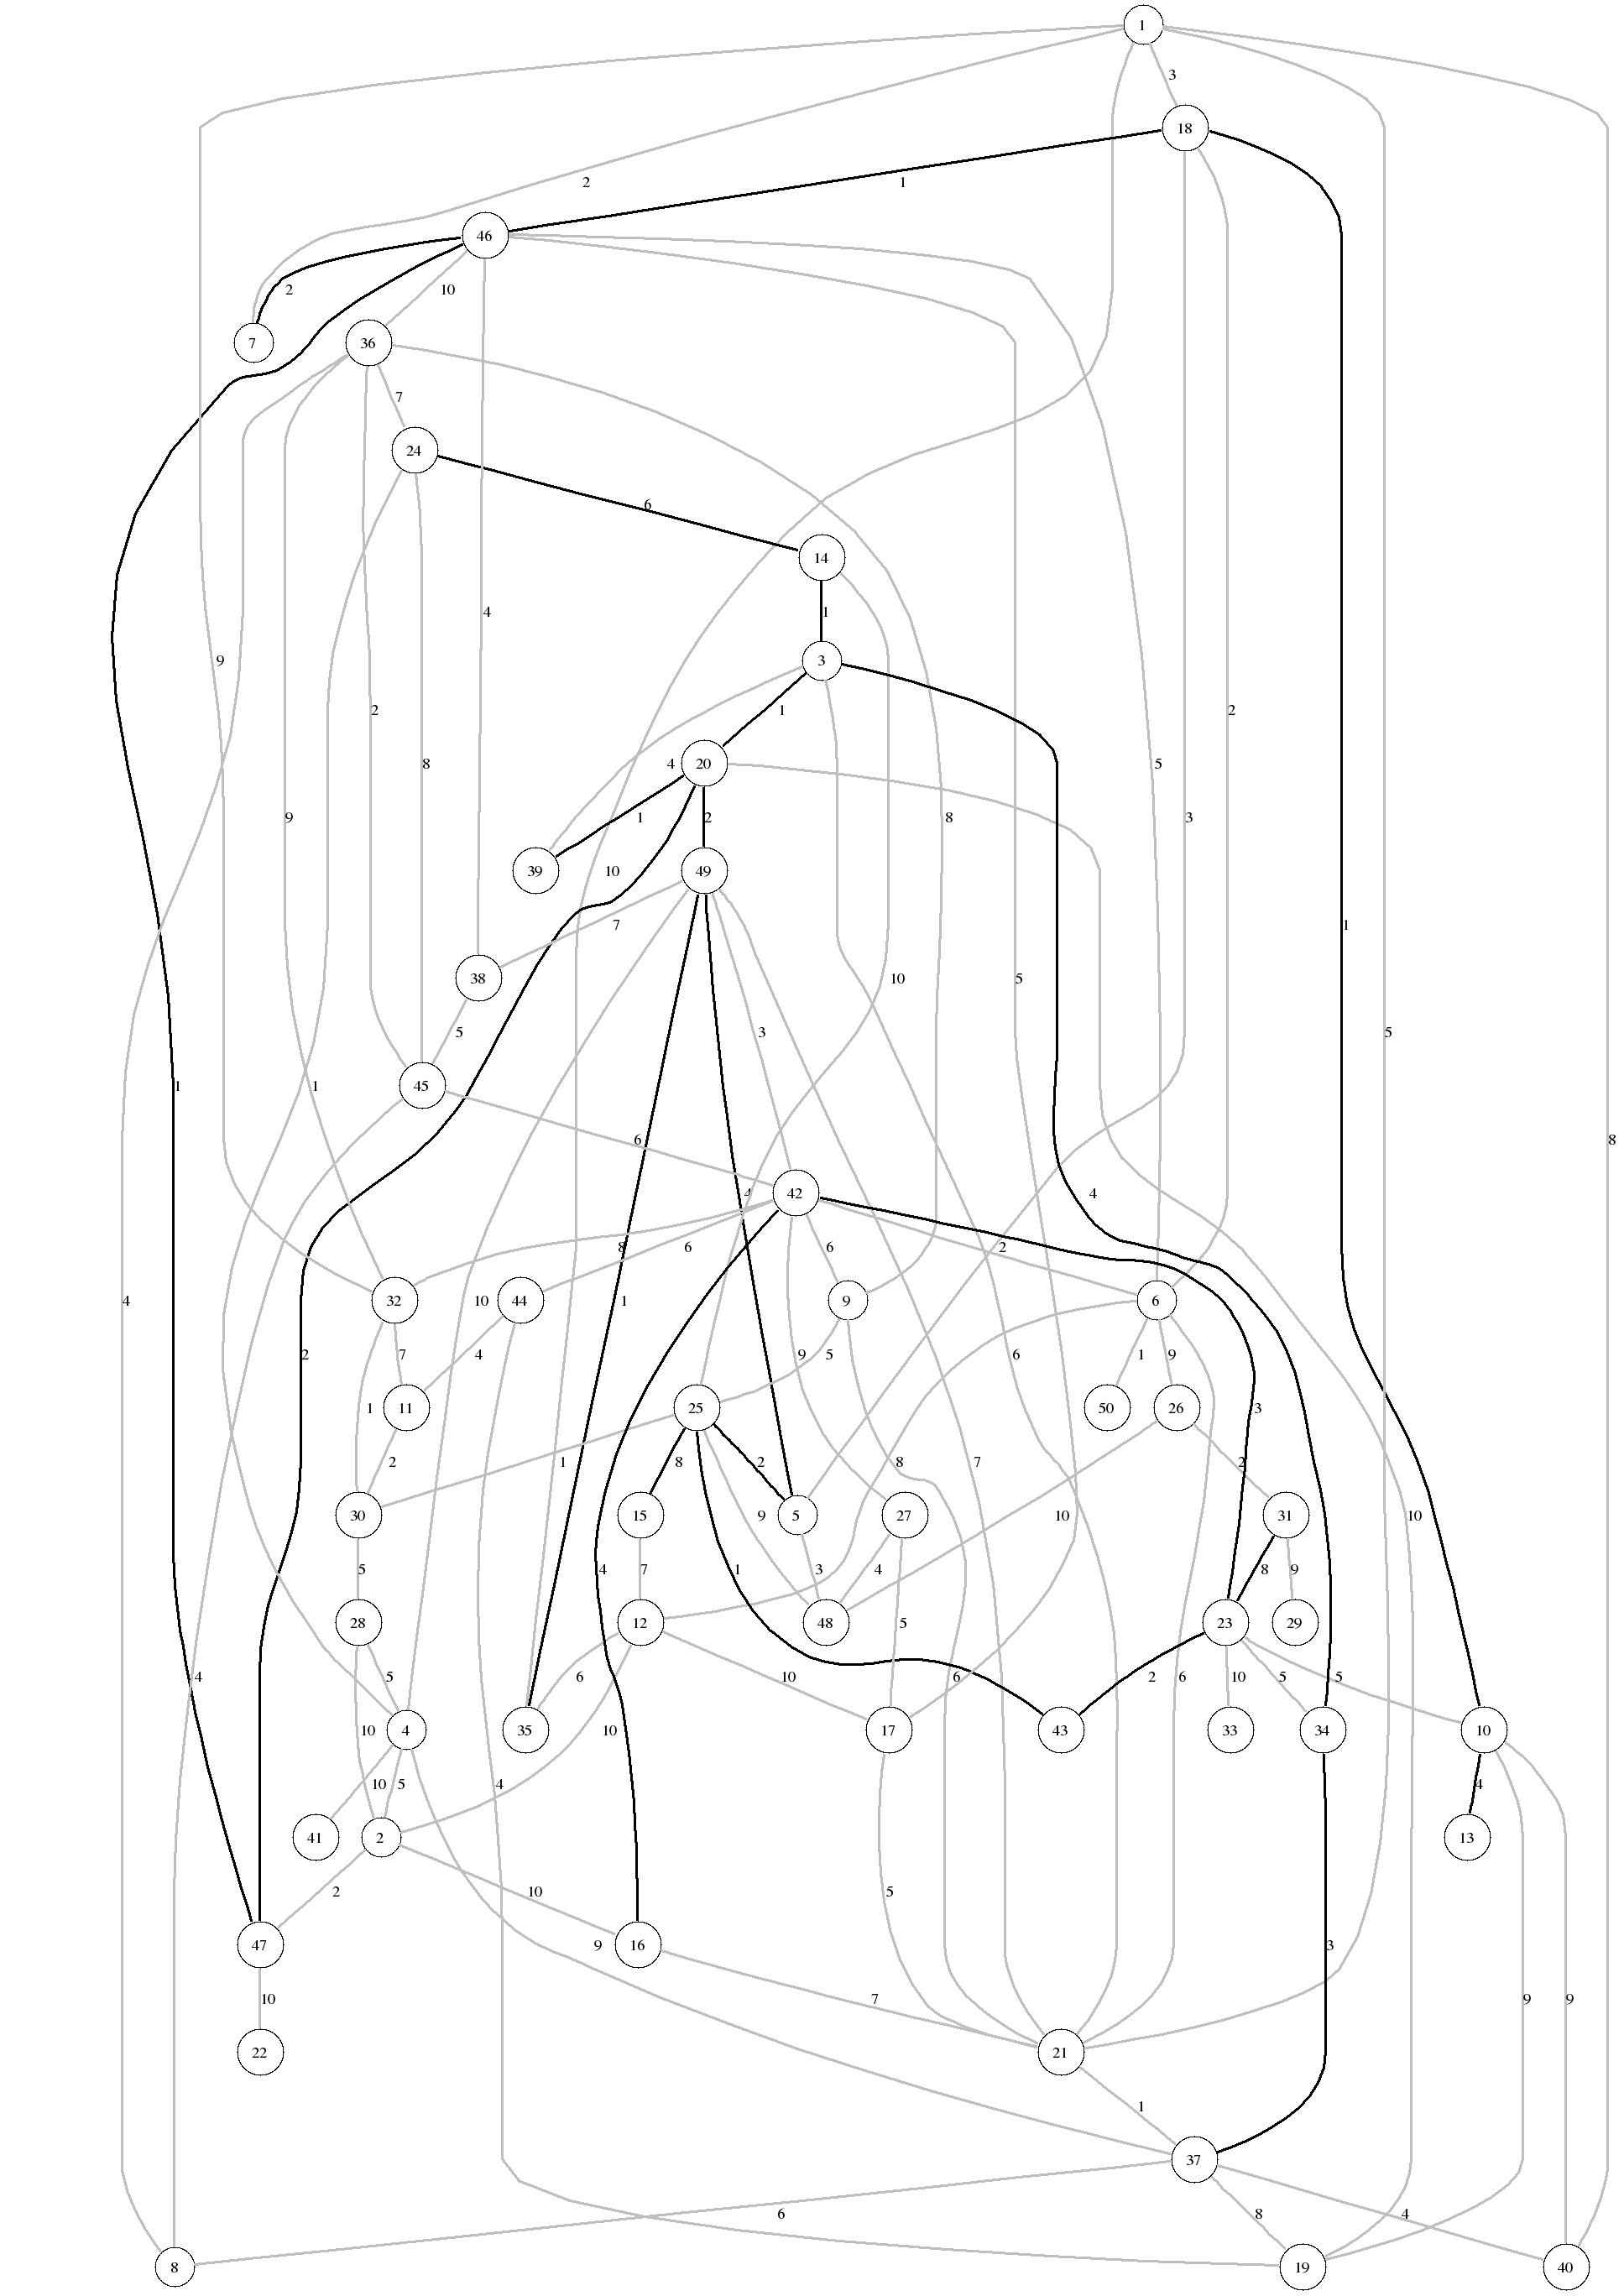
\includegraphics[keepaspectratio=true,width=\linewidth,height=\textheight]{b05.eps}

\section*{Running Time}
KMB is a heuristic algorithm for finding Steiner trees with a worst case time
complexity of $O(|S||V|^{2})$. It is guaranteed to yield a tree that spans $S$ with a
total distance on its edges no more than $2(1 - \frac{1}{l})$ times that of the optimal
tree, where $l$ is the number of leaves in the optimal tree. The paper \textit{Multicasting
for High-Bandwidth Delay-Sensitive Multimedia Applications}\cite{ks:kpp} put the
running time at $O(n^{3})$ to find the the shortest paths and $O(n^{2} \log n)$ for
determining the tree where $n$ is the number of nodes in the graph.\\*[1Em]

Our implementation ran with zero run time on all the graphs we tested and
made measurement in seconds difficult.

\section*{Conclusion}
The beauty of the KMB graph is its ability to reduce a tough problem using two
well-known algorithms to achieve a close approximation of a Steiner tree. This 
project really expanded our knowledge of C++ and graph algorithms, and we hope our
implementation is capable of further exploring the KMB algorithm with any undirected
graph.

\end{raggedright}
\nocite{ks:pzh}
\bibliography{report}
\bibliographystyle{plain}
\end{document}


